%!TEX root = thesis.tex
%%%%%%%%%%%%%%%%%%%%%
%
%
%%%%%%%%%%%%%%%%%%%%%%%%%%%%%%%%%
%%%%%%%%%%%%%%%%%%%%%%%%%%%%%%%%%
\chapter{Matrix product states}
\label{sec:matrix_product_states}
%%%%%%%%%%%%%%%%%%%%%%%%%%%%%%%%%
%%%%%%%%%%%%%%%%%%%%%%%%%%%%%%%%%
The analytical treatment as presented in the previous chapter relies on a heavy line of approximations (which are sometimes very hard to justify on a rigorous level).
One of the most crucial consequences is that quantitative deviations occur if the interactions are comparable to the kinetic bandwidth.
This not only restricts heavily the strict validity region of the effective field theory, it sometimes even contradicts the relevancy predictions of the RG.
For instance, the spin-$1/2$ XXZ chain shows a sine-Gordon term with $\beta=4$, relevant for $K<1/2$.
Such small Luttinger parameter requires a very strong nearest neighbor interactions compatible with the system's bandwidth.
Naturally, we expect quantitative deviations from the Luttinger liquid predictions in such regions and must rely on numerical tools to resolve the microscopic details of these strongly correlated phases of matter.
In this chapter, I will provide the essentials to get acquainted with the concepts of tensor networks, in particular with matrix product states (MPS).
\\

First, I give a basic introduction to tensor networks and explain the intuitive concept of renormalization through a truncation of the auxiliary dimension of these structures.
Second, I review the concept of ``area laws'' -- a statement about the structure of quantum correlations of gapped and short-ranged Hamiltonians -- and connect it to the properties of tensor networks.
I will then present renormalization strategies which provide variational search algorithms to target ground (and low-lying excited) states and continue by presenting a simple yet effective time-evolution algorithm in the framework of MPS.
As a conclusion, I describe the exploit of abelian symmetries in the numerical techniques which in general reduces the overall computational complexity.
%
%
%%%%%%%%%%%%%%%%%%%%%%%%%%%
\section{Tensor networks}
\label{sec:tensor_networks}
%%%%%%%%%%%%%%%%%%%%%%%%%%%
A tensor is a collection of complex numbers in multidimensional arrays.
Its rank is given by the number of indices: for instance, scalar values are of rank zero, vectors of rank one and matrices of rank two.
Tensor networks are in general contractions of many tensors and as such it is customary to define graphical representations which display its fundamental structure, i.e. its rank.
The most common convention is to represent a tensor object as a circle, triangle, hourglass or rectangle with as many legs as the tensor has indices.
It is then easy to sketch the tensor contraction of a simple matrix-matrix multiplication as
\begin{align}
    C_{i,j}=A_{ik}B_{kj}\equiv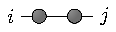
\includegraphics[valign=c]{figures/MatrixMultiplication.pdf},
\end{align}
in which I conveniently use the sum convention.
Switching from formulas to graphical notation may become interesting when considering larger tensor networks.
One easy example is a trace of many matrices, which can be sketched as a circle contraction.
\begin{align}
    \tr\brlr{ABCDEF} \equiv 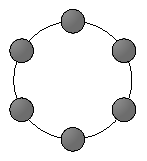
\includegraphics[valign=c]{figures/MatrixTrace.pdf}.
\end{align}
For more complex contractions containing tensors of higher ranks, it is important to optimize the sequence of contractions to reduce the overall computational cost to a minimum.
For instance, in \cref{fig:contraction_sequences} two different sequences of contractions obviously result in the same outcome, but the overall complexity class is different.
Assume each leg has dimension $m$, then sequence $S_1$ is $O(m^4)$ whereas sequence $S_2$ is $O(m^4)$.
\begin{figure}
    \centering
    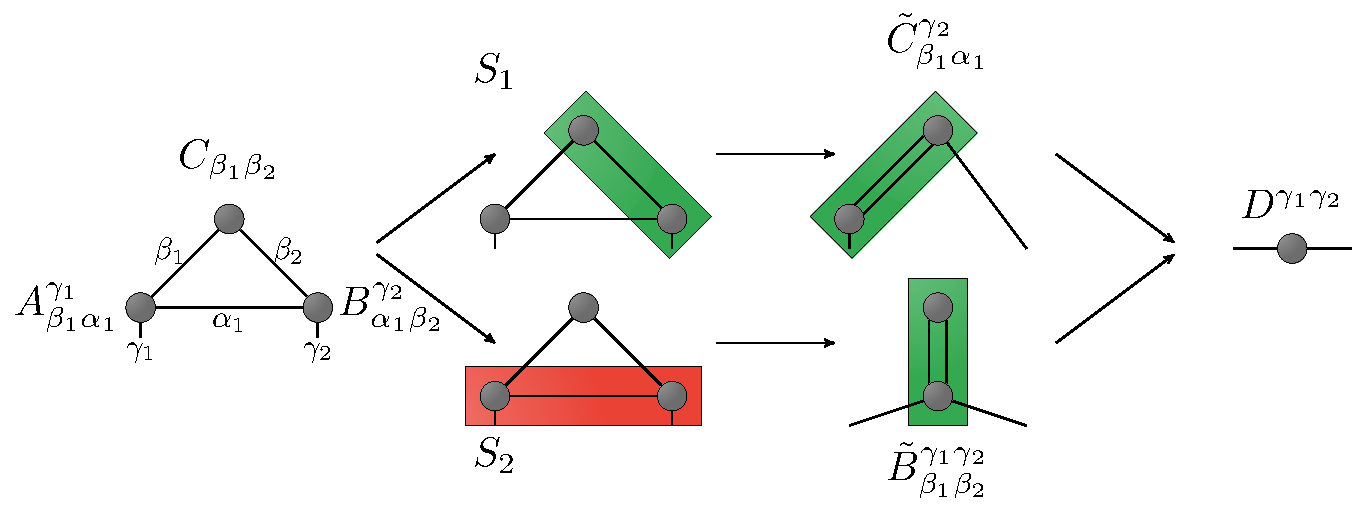
\includegraphics[width=0.8\textwidth]{figures/ComplexContraction1.pdf}
    \caption{Different complexity classes for the same contraction, but different sequences. Assume each index has dimension $m$, then the green contractions are $O(m^4)$, but red is $O(m^5)$. Hence, sequence $1$ requires less multiplications compared to $2$ and is thus less prone to numerical truncation errors.}
    \label{fig:contraction_sequences}
\end{figure}
A triangle representation may make sense to indicate a tensor being an isometry.
For instance, consider the two isometries $U$, $V^\dag$ of a generic singular value decomposition (SVD) $M = U \Lambda V^\dag$: they contain the left- and right-singular vectors of $M$ and are thus semi-unitaries, i.e.
\begin{align}
    U^\dag U^\pdag = \mathbb1,
    \quad
    V^\dag V^\pdag = \mathbb1.
\end{align}
In graphical notation, the identity matrix is represented as a straight line as it does neither stretch nor rotate the entries of a tensor.
The previous equation can thus be recast to
\begin{align}
    U^\dag U^\pdag \equiv 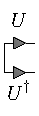
\includegraphics[valign=c]{figures/right_isometry.pdf} = 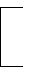
\includegraphics[valign=c]{figures/right_identity.pdf}\,,
    \qquad
    V^\dag V^\pdag \equiv 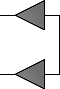
\includegraphics[valign=c]{figures/left_isometry.pdf} = 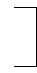
\includegraphics[valign=c]{figures/left_identity.pdf}\,.
    \label{eq:isometries}
\end{align}
A simple squared unitary matrix is orthogonal with respect to both left/right multiplication with its adjoint and as such can be represented as a hourglass.
The SVD of a normal matrix $M$ can be recast to the graphical notation
\begin{align}
    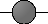
\includegraphics[valign=c]{figures/matrix.pdf}
    \equiv M = U \Lambda V^\dag \equiv
    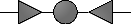
\includegraphics[valign=c]{figures/svd.pdf}\,.
\end{align}
Let me now introduce probably the most important decomposition applied in tensor networks -- the generalized version of the SVD for rank $n$ tensors:
(i) the rank $n$ array has to be reduced to a rank $2$ object, i.e. a matrix.
This transformation (which must be a bijection) is commonly called tensor reshaping and is understood in graphical notation as a fusion of multiple tensor legs.
(ii) The matrix then is decomposed through a standard SVD, followed by (iii) the restoration of the original rank $n$ object through the inverse reshaping applied in step (i).
The identity relation between the original and decomposed tensor is assured by the inverse of (i).
For a practical example, consider a rank $n$ tensor $T$ which is graphically depicted by $n$ legs (labelled by increasing numbers from $1,...,n$ from left to right).
To perform a SVD between the bipartition after leg $j$, the tensor is reshaped to a matrix through a fusion of legs $1,...,j$ and $j+1,...,n$ prior to the performed SVD, after which the original rank is restored.
In particular, the sequence of identities reads
% \begin{align}
%     % 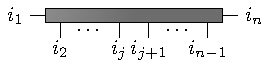
\includegraphics[valign=c]{figures/rankntensor.pdf}
%     % =
%     T_{i_1,i_n}^{i_2,\dots,i_j,i_{j+1},\dots,i_{n-1}}
%     &\overset{(i)}{=}
%     f^{-1}\circ T_{(i_1,\dots,i_j),(i_{j+1},\dots,i_n)}
%     \\
%     &\overset{(ii)}{=}
%     f^{-1}\circ\sum_k U^\pdag_{(i_1,\dots,i_j),k}S^\pdag_{k}{V^\dag}_{k,(i_{j+1},\dots,i_n)}
%     \\
%     &\overset{(iii)}{=}
%     \sum_kU_{i_1,k}^{i_2,\dots,i_j}S^\pdag_{k}{V^\dag}_{k,i_n}^{i_{j+1},\dots,i_{n-1}},
% \end{align}
\begin{align}
    T_{i_1,i_n}^{i_2,\dots,i_j,i_{j+1},\dots,i_{n-1}}
    \equiv&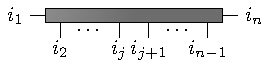
\includegraphics[valign=c]{figures/rankntensor.pdf},
    \\
    \overset{(i)}{=}&
    f^{-1}\circ
    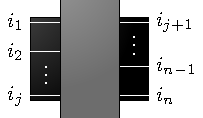
\includegraphics[valign=c]{figures/reshaping.pdf}
    \equiv
    f^{-1}\circ U^\pdag_{(i_1,\dots,i_j),k}\Lambda^\pdag_{k}V^\dag_{k,(i_{j+1},\dots,i_n)},
    \\
    \overset{(ii)}{=}&
    f^{-1}\circ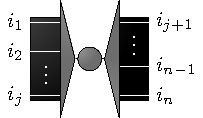
\includegraphics[valign=c]{figures/bigsvd.pdf}
    \equiv
    f^{-1}\circ U^\pdag_{(i_1,\dots,i_j),k}\Lambda^\pdag_{k}V^\dag_{k,(i_{j+1},\dots,i_n)},
    \\
    \overset{(iii)}{=}&
    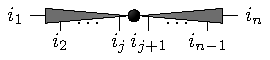
\includegraphics[valign=c]{figures/rankntensor_decomposed.pdf}
    \equiv
    U_{i_1,k}^{\pdag i_2,\dots,i_j}\Lambda^\pdag_{k}{V^\dag}^{i_{j+1},\dots,i_{n-1}}_{k,i_n},
    \label{eq:SVD_generalized}
\end{align}
in which $f^{-1}$ denotes the inverse of the tensor reshaping / leg fusion, and Einstein notation implies the tensor contraction contraction with summed index $k$.
In the equations above, it is assumed that the applied SVD is compact: $\Lambda$ is a square and diagonal matrix containing the nonzero singular values, such that $\Lambda_{ij}\equiv s_i\delta_{ij}$.
\\

To get acquainted with the use of tensors in a more practical sense, let us aim to understand some of the described concepts in the context of two-dimensional pictures.
If we assume the picture to be rasterized in an equidistant manner using square pixels, the RGB-entries of the pixel can be collected in a 3D array of the form
\begin{align}
    P_{y,x}^{c}\equiv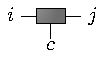
\includegraphics[valign=c]{figures/tensor_picture.pdf}.
\end{align}
The position of the pixel is encoded by the indices $y,x$ and $c$ represents a leg containing the RGB-values (e.g., $c\in\{1,2,3\}\equiv\{r,g,b\}$).
Using the concept of the generalized SVD, we can decompose the tensor $P$ into two semi-unitaries $U,V^\dag$ and a vector $S_k$ containing the singular values of the bipartition.
There exist three different bipartitions: (a) $P_{(y,x),c}$, (b) $P_{(y,c),x}$ and (c) $P_{y,(x,c)}$.
(b) and (c) are equivalent up to a transposition of the original object, therefore leaving two truly different decompositions, (a) and (b).
The bipartition (a) targets a decomposition between $(y,x)$ and $c$ whereas (b) targets a decomposition between $y$ and $(x,c)$.
Strategy (a) thus aims to truncate the color degree of freedom, which is not very useful due to the low dimensionality of the $c$ leg (there are only $3$ nonzero singular values to begin with), such that I will focus entirely on the decomposition of (b).
\\

\begin{figure}
    \centering
    \subfigure[]{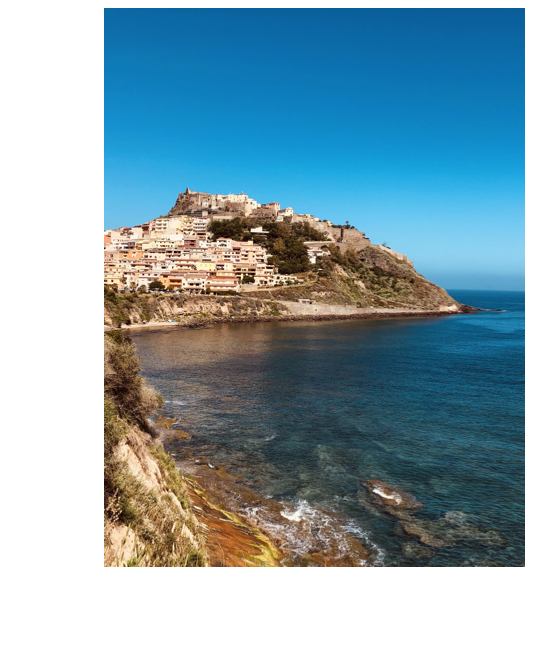
\includegraphics{figures/SVD_uncompressed.png}}
    \hfil
    \subfigure[]{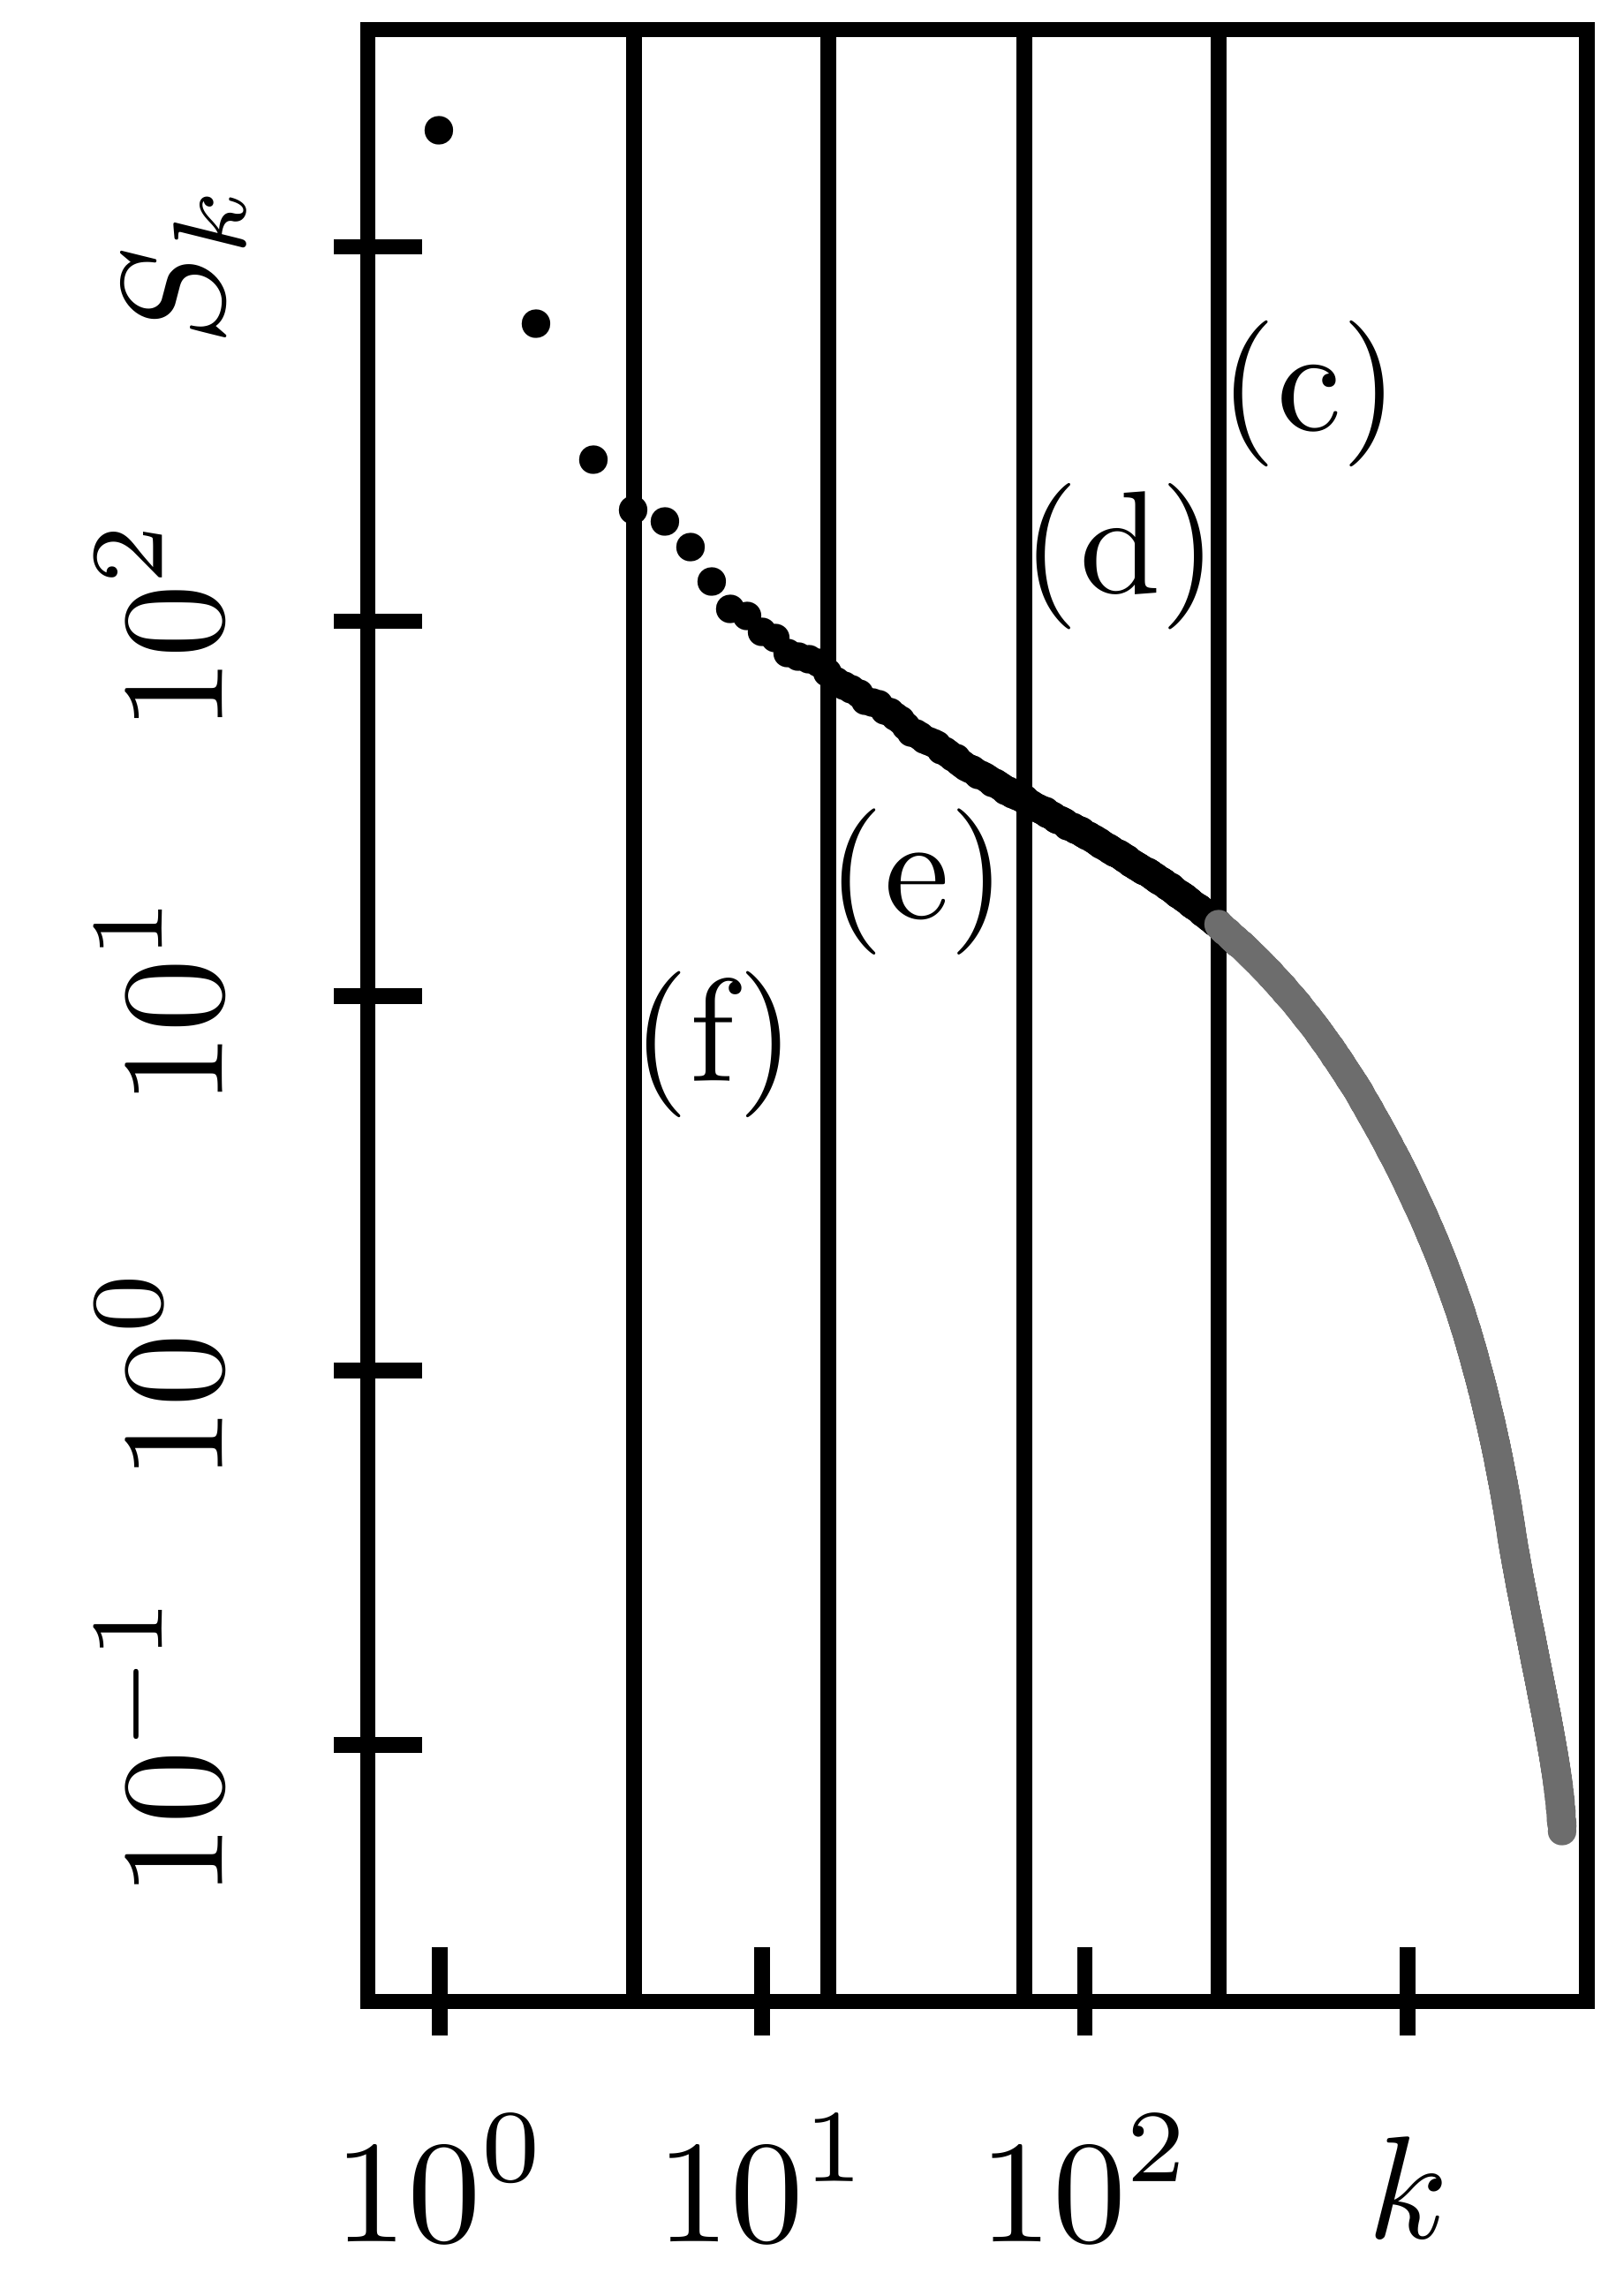
\includegraphics{figures/beach_singular_values.png}}
    \hfil
    \subfigure[]{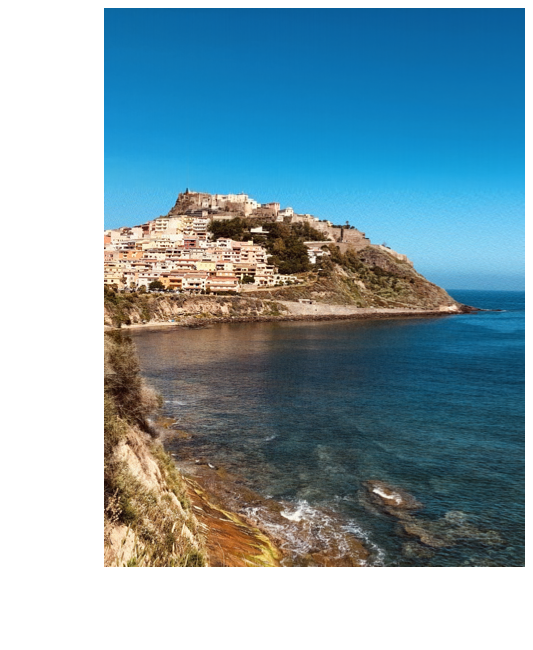
\includegraphics{figures/SVD_compressed.png}}
    \caption{(a) Uncompressed picture of Castelsardo (Sardinia, IT).
    The digital picture consists of $n_y\times n_x=3024\times2276$ pixels. (b) Singular values of the matrix $P_{i,(jc)}$ representing the picture. (c) Keeping the $250$ largest singular values still yields a good approximation of the uncompressed picture and requires only $19.3\%$ of the original storage space.}
    \label{fig:svd_image_compression}
\end{figure}
If the singular/spectral values are ordered, a truncation of the $\Lambda$ matrix neglects subdominant left and right eigenvectors of the original object and as such approximates the original matrix.
In case of a subsequent normalization to the original trace, the truncation process can be understood as a compression or tensor renormalization scheme.
The number of singular values kept in the approximation is thus naturally linked to the accuracy of the numerical renormalization.
Assume the picture to be of dimensions $\dim(P)=p_y\times p_x\times 3$, then keeping $m$ singular values implies that we need to store only a fraction of the matrices $U$ and $V^\dag$ to approximate the original picture $P$.
Assuming that the matrix $M\equiv \{P_{y,(x,c)}\}_{y,x,c}$ is of dimension $n_y=p_y$ times $n_x=3p_x$, the following visualization highlights the SVD
\begin{align}
    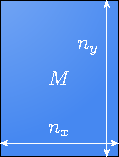
\includegraphics[valign=c]{figures/svd_mmat.pdf}
    =
    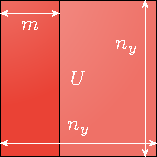
\includegraphics[valign=c]{figures/svd_umat.pdf}
    \
    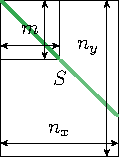
\includegraphics[valign=c]{figures/svd_smat.pdf}
    \
    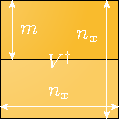
\includegraphics[valign=c]{figures/svd_vmat.pdf}.
    \label{eq:compression_scheme}
\end{align}
If we limit to $m$ spectral values, we only need to store $n_y\cdot m$ elements from $U$, $m$ singular values and $m\cdot n_x$ elements from $V^\dag$.
In total, we thus arrive at a compression rate
\begin{align}
    C_m = \frac{(n_x+n_y+1)m}{n_x n_y},
\end{align}
which allows for a high compression in case of a large and dense matrix $M$.
To give an example, I present the impact of compression in \cref{fig:svd_image_compression}.
Panel (a) denotes an uncompressed picture, the singular values of the digital picture presented in (b), and the result of keeping $250$ singular values as an approximation to the full picture, presented in (c).
The approximated picture yields a compression rate of roughly $19\%$, and visible differences to the original are negligible (if you look closely, the compressed figure appears to have some ``noise'' in the nice color gradient of the sky).
\\

The depicted compression scheme can actually be applied to quantum states.
Recall that any state can be expressed by a set of $L$ good quantum numbers, such that
\begin{align}
    \ket{\psi} = \sum_{i_1,i_2,\dots,i_L}C({i_1,i_2,\dots,i_L})\ket{i_1,i_2,\dots,i_L}
    \label{eq:generic_state}
\end{align}
and the collection of all $\ket{i_1,i_2,\dots,i_L}$ form a complete and orthonormal basis.
Note that the $L$-dimensional array $C$ depends on all internal quantum numbers and is thus exponentially large in the system size $L$ and the dimension of the quantum numbers $i_j$.
By the visual conventions, we may imagine the coefficients $C$ as a rank $L$ tensor, similar to the tensor $T$ discussed in \cref{eq:SVD_generalized}
\begin{align}
    C(i_1,i_2,\dots,i_L) = C^{i_1,i_2,\dots,i_L} \equiv  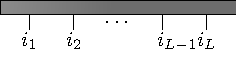
\includegraphics[valign=c]{figures/arbitrary_wavefunction.pdf}.
\end{align}
This allows to apply the generalized SVD in a sequential manner:
Starting with the decomposition spanned by the bipartition of the first (last) leg, keeping the left (right) isometry and shifting the right (left) isometry to the adjacent leg position, is possible to decompose $C$ into a product of isometries with a single $\Lambda$ matrix in between two arbitrary leg positions $\ell,\ell+1$.
The necessary decomposition sequence is most easily reformulated in graphical notation
\begin{align}
    C^{i_1,i_2,\dots,i_L} \equiv 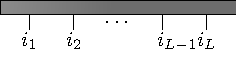
\includegraphics[valign=c]{figures/arbitrary_wavefunction.pdf}
    =
    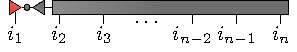
\includegraphics[valign=c]{figures/arbitrary_wavefunction_partially_decomposed_1.pdf}
    \\
    =
    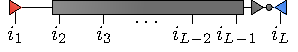
\includegraphics[valign=c]{figures/arbitrary_wavefunction_partially_decomposed_2.pdf}
    \\
    =
    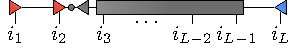
\includegraphics[valign=c]{figures/arbitrary_wavefunction_partially_decomposed_3.pdf}
    \\
    =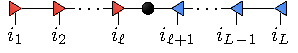
\includegraphics[valign=c]{figures/arbitrary_wavefunction_decomposed.pdf}
    \label{eq:move_the_lambda_matrix}
\end{align}
in which at each step the three gray tensors are contracted before performing the next SVD.
This particular decomposition of a generic quantum state, i.e.
\begin{align}
    C^{i_1,i_2,\dots,i_L} \equiv 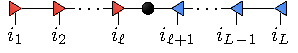
\includegraphics[valign=c]{figures/arbitrary_wavefunction_decomposed.pdf}
\end{align}
is called the canonical form of an MPS.
In other words, it represents the Schmidt decomposition of the state $\ket{\psi}$ in the subspaces $\HS_{A(\ell)}$ and $\HS_{B(\ell)}$ spanned by the first $\ell$ and last $L-\ell$ quantum numbers i.e.
\begin{align}
    \ket\psi = \sum_{\bm i} C^{\bm i}\ket{\bm i} = \sum_{k}s_{k}(\ell)\ket{\psi_{A(\ell),k}}
    \ket{\psi_{B(\ell),k}}
\end{align}
in which the transformed states $\ket{\psi_{A/B,k}}$ are given by the SVD-decomposed coefficient matrix
\begin{align}
    \ket{\psi_{A(\ell),k}}
    &=
    U^{i_1}_{k_1} U^{i_2}_{k_1,k_2}U^{i_3}_{k_2,k_3}\dots U^{i_\ell}_{k_{\ell-1},k}\ket{i_1,i_2,i_3,\dots,i_j}
    =\prod_{k=1}^\ell U^{[i_k]}\ket{i_1,\dots,i_\ell},\\
    %
    \ket{\psi_{B(\ell),k}}
    &=
    {V^\dag}^{i_{\ell+1}}_{k,k_{\ell+1}} {V^\dag}^{i_{\ell+2}}_{k_{\ell+1},k_{\ell+2}}\dots {V^\dag}^{i_L}_{k_{L-1}}\ket{i_{\ell+1},\dots,i_L}
    =
    \prod_{k=\ell+1}^L V^{\dag[i_k]}\ket{i_{\ell+1},\dots,i_L}.
\end{align}
Please note that I used the sum convention for convenience.
It is now obvious that (i) any quantum state can be decomposed into an MPS, (ii) that each MPS can be brought into the canonical form and (iii) that MPS have a large gauge degree of freedom.
Point (iii) is clear from the fact that one may sandwich infinitely many identities in the MPS (each written as a product of two unitary matrices) which may in general rotate the colored isometry tensors, but leave the overall state invariant.
\\


To understand the influence of the compression scheme, consider the way a generic density matrix is expressed in terms of a canonical MPS:
\begin{align}
    \hat\rho = \ket{\psi}\bra{\psi} = \sum_{k,k'}s_ks_{k'}\ket{\psi_{A,k},\psi_{B,k}}\bra{\psi_{A,k'},\psi_{B,k'}}.
\end{align}
Now imagine to compute the reduced density matrix of a bipartition formed by a block $A(\ell)$ of the first $\ell$ quantum numbers and a block $B(\ell)$ of the remaining ones (same as before).
A trace over the complement states of the partition $A/B$ gives the reduced density matrix in block $A/B$, i.e.
\begin{align}
    \hat\rho_A = \tr_B(\hat\rho)
    &=
    \sum_{k,k',k''}
    s_ks_{k'}
    \braket{\psi_{B,k''}|\psi_{A,k},\psi_{B,k}}\braket{\psi_{A,k'},\psi_{B,k'}|\psi_{B,k''}}
    =
    \sum_k s_k^2 \ket{\psi_{A,k}}\bra{\psi_{A,k}},\nonumber\\
    %
    \hat\rho_B = \tr_A(\hat\rho)
    &=
    \sum_k s_k^2 \ket{\psi_{B,k}}\bra{\psi_{B,k}}.
\end{align}
Note that normalization of the quantum state $\ket\psi$ implies $\tr\rho=\sum_k s_k^2=1$ and $s_k^2$ can be interpreted as the probability of state $\ket{\psi_{A/B,k}}$ contributing to the reduced density matrix $\hat\rho_{A/B}$.
The reduced density matrix is thus diagonal in the Schmidt decomposition, and solely determined by the spectral values $s_k$.
Imagine now to approximate the state $\ket\psi$ with a state $\ket{\psi'}$ by limiting the number of different $s_k$ in the bipartition $A,B$ such that the $m$ largest spectral values are kept in $\ket{\psi'}$ and the rest is set to zero.
Normalization of the state $\ket{\psi'}$ requires that $\sum_{k=1}^m {s'_k}^2$ must be renormalized to unity, which is satisfied if $s_k'=s_k/\sqrt{\sum_{l=1}^m s_l^2}$.
The threshold $m$ is thus directly related to approximating the reduced density matrix $\hat \rho_{A/B}$ with the $m$ most likely states in the Schmidt decomposition of a given bipartition $A/B$.
Please note that $s_k\equiv s_k(\ell)$ refers to the $k$'th singular value of a particular bipartition $A(\ell)/B(\ell)$, which considers the first/last $\ell/L-\ell$ quantum numbers.
% Therefore, it can be appropriate to denote this dependence also in the spectral values if needed, i.e. $s_k = s_k(\ell)$.
If we keep the $m$ largest singular values $s_k(\ell)$, $k\in\{1,2,\dots,m\}$ for any block size $\ell$, $m$ is a global property of MPS called the bond dimension.
\\

Density matrices are naturally related to the generalized Gibbs entropy for quantum states
\begin{align}
    S_1(\ell) = -\tr(\hat\rho_A\log\hat\rho_A) = -\tr(\hat\rho_B\log\hat\rho_B) = -\sum_k s^2_k\log(s^2_k)
\end{align}
which is a straightforward measure for the shared information between the bipartition, in information theory perspectives often called Shannon entropy of communication.
In this context, $-\log(s^2_k)$ is understood as the information content (or surprisal) of the Schmidt state, and $S_1$ is simply the expectation value of surprisal.
Such definition is readily understood from an experimentalist's point of view: measuring a state of very low spectral weight are surprizing, whereas likely quantum states bear a low surprise.
In a quantum physics audience, the entropy $S_1$ is commonly referred to as von Neumann entropy, and I denote it as $S_1$ because of its relation to the Rényi entropy -- a generalized version of the Shannon entropy
\begin{align}
    S_\alpha(\ell) = \frac{1}{1-\alpha}\tr\log\rho^\alpha_A
\end{align}
in the limit $\alpha\rightarrow1$.
The derivation of the limit is infrequently presented in the literature, but straightforward by using the Schmidt decomposition and L'Hôpital's rule
\begin{align}
    S_1(\ell)
    =
    \lim_{\alpha\rightarrow1}\frac1{1-\alpha}\tr\log\hat\rho_A^\alpha
    =
    -\lim_{\alpha\rightarrow1}\partial_\alpha\log\sum_k s_k^{2\alpha}
    =
    -\lim_{\alpha\rightarrow1}\frac{\sum_k\partial_\alpha s_k^{2\alpha}}{\sum_k s_k^{2\alpha}}
    =
    -\lim_{\alpha\rightarrow1}\sum_k \re^{\alpha\log s_k^2}
    \\
    =
    -\lim_{\alpha\rightarrow1}\sum_k \re^{\alpha\log s_k^2}\log s_k^2
    =
    -\sum_k s_k^2\log s_k^2
    =
    -\tr \hat\rho_A\log\hat\rho_A.
\end{align}
In conclusion, using MPS techniques in the canonical form provides immediate access to the information content of a given bipartition.
Note that the maximum entropy of an MPS is always restricted by the bond dimension $m$, i.e. $S_1(\ell)<\log(m)$.
\\

Let us now understand the action of operators in the basis of MPS.
Consider a local operator acting on site $q$, which can be written in general as $\hat o_q = \sum_{i_q',i_q''}o_{i_q',i_q''}\ket{i_q'}\bra{i_q''}$.
Its action on the canonical form of an MPS can be expressed as
\begin{align}
    \hat o_q\ket\psi &= \sum_{i_1,i_2,\dots,i_q,\dots,i_L}\sum_{i_q'}o_{i_q',i_q} C^{i_1,i_2,\dots,i_q,\dots,i_L}\ket{i_1,i_2,\dots,i_{q-1},i_q',i_{q+1},\dots,i_L}
    \\
    &= \sum_{i_1,i_2,\dots,i_L}\tilde C^{i_1,i_2,\dots,i_L}\ket{i_1,i_2,\dots,i_L}
\end{align}
and we note that it leaves the overall form of the MPS invariant.
In particular, it acts as a contraction between the $o$-matrix and the $q$'th vertical leg of the $C$-tensor, according to
\begin{align}
    \tilde C^{i_1,i_2,\dots,i_L} = \sum_{i_q'}o_{i_q,i_q'}C^{i_1,i_2,\dots,i_q',\dots,i_L}.
\end{align}
Therefore, we can represent any local operator as a rank-$2$ tensor composed by the matrix elements of $\hat o$.
The same reasoning applies for operators acting on $p$ sites -- they are represented by rank-$2p$ tensors containing the entries of the matrix elements, contracted with the $p$ corresponding vertical links of the $C$-tensor.
Such objects are then called matrix product operator (MPO) and allow the efficient representation of generic Hamiltonians.
This is particularly easy to see as the Hamiltonian is simply a sum of products of local operators, which each have an MPO representation.
Consider the simple example of the Ising model with the following Hamiltonian
\begin{align}
    \hat H = \hat H_{h} + \hat H_{J},
    \quad
    \hat H_{J} = J\sum_{i=1}^{L-1}\hat X_i \hat X_{i+1},
    \quad
    \hat H_{h} = h\sum_{i=1}^{L}\hat Z_i
\end{align}
in which $\hat X/\hat Y/\hat Z$ denote the spin-1/2 Pauli operators.
They have the following representations
\begin{align}
    \hat X = \ket{\uparrow}\bra{\downarrow} + \ket{\downarrow}\bra{\uparrow},
    \quad
    \hat Y = -\ri \ket{\uparrow}\bra{\downarrow} + \ri\ket{\downarrow}\bra{\uparrow},
    \quad
    \hat Z = \ket{\uparrow}\bra{\uparrow} - \ket{\downarrow}\bra{\downarrow}.
\end{align}
Note that the Hamiltonian can be recast into a product of bulk $i\neq1,L$ operators of the form
\begin{align}
    \hat W^{[i]} =
    \begin{pmatrix}
        \mathbb 1_i & \hat X_i & \hat Z_i\\
         0 & 0 & \hat X_i\\
        0 & 0 & \mathbb 1_i\\
    \end{pmatrix}
\end{align}
representing a set of local operators acting locally on a single site.
The multiplication of the $\hat W$ matrix operators does not yield the desired result immediately,
% \begin{align}
%     \hat W_{i}\hat W_{i+1} =
%     \begin{pmatrix}
%         \mathbb1 & \hat X_{i+1} & \hat X_i\hat X_{i+1} + \hat Z_i + \hat Z_{i+1} \\
%         0 & 0 & \hat X_{i}\\
%         0 & 0 & \mathbb1
%     \end{pmatrix},
% \end{align}
which is readily solved by a slight modification of the boundary tensors
\begin{align}
    \hat W^{[1]} =
    \begin{pmatrix}
        \mathbb 1 & 0 & 0
    \end{pmatrix}
    \begin{pmatrix}
        \mathbb 1_1 & \hat X_1 & \hat Z_1\\
         0 & 0 & \hat X_1\\
        0 & 0 & \mathbb 1_1\\
    \end{pmatrix}
    =
    \begin{pmatrix}
        \mathbb 1 & \hat X_1 & \hat Z_1
    \end{pmatrix}
    ,
    \quad
    \hat W^{[L]} =
    \begin{pmatrix}
        \mathbb 1_L & \hat X_L & \hat Z_L\\
         0 & 0 & \hat X_L\\
        0 & 0 & \mathbb 1_L\\
    \end{pmatrix}
    \begin{pmatrix}
        0 \\ 0 \\ \mathbb 1
    \end{pmatrix}
    \begin{pmatrix}
        \hat Z_L\\
        \hat X_L\\
        \mathbb 1_L\\
    \end{pmatrix}
\end{align}
such that the global Hamiltonian is given by the product
% \begin{align}
%     \hat X_i\hat X_{i+1} + \hat Z_i + \hat Z_{i+1} = \hat W_l \hat W_i \hat W_{i+1} \hat W_r
% \end{align}
% and as such
\begin{align}
    \hat H = \prod_{i=1}^{L}\hat W^{[i]}.
\end{align}
Since $\hat W$ contains a set of local operators which each have an MPO representation, the above operator expression acting on a state $\ket\psi$ is nothing but tensor contraction in which the local rank-$2$ tensors representing the action of the spin operators are promoted to a rank-$4$ MPO $W$ containing the matrix elements of $\hat W$.
In particular, one obtains
\begin{align}
    W =
    \begin{pmatrix}
        \mathbb 1 & X & Z \\
        0 & 0 & X \\
        0 & 0 & \mathbb 1
    \end{pmatrix}
    ,
    \quad
    X =
    \begin{pmatrix}
        0 & 1 \\
        1 & 0
    \end{pmatrix}
    ,
    \quad
    Y =
    \begin{pmatrix}
        0 & -\ri \\
        \ri & 0
    \end{pmatrix}
    ,
    \quad
    Z =
    \begin{pmatrix}
        1 & 0 \\
        0 & -1
    \end{pmatrix}
    .
\end{align}
The MPO representation $W$ of the Hamiltonian $\hat H$ is very versatile -- any Hamiltonian can be recast into a set of matrix product operators that are upper triangular, even if the interactions are long-ranged or spacially dependent, e.g. in the case of disorder.
%
%
%%%%%%%%%%%%%%%%%%%%%%%%%%%%%%%%%%%%%%%%%%%
\section{Variational ground state search}
\label{sec:variational_ground_state_search}
%%%%%%%%%%%%%%%%%%%%%%%%%%%%%%%%%%%%%%%%%%%
%
%
The original variational ground state search is formalized in the density matrix renormalization group (DMRG), introduced by Steven White in 1992~\cite{White1992}.
In it's essence, it is a numerical optimization scheme targetting the low energy sector of a given system.
Nowadays, it is understood as an MPS Ansatz of the trial wavefunction in which at each iteration a few local tensors (in most cases one or two) are variationally optimized.
For the numerical simulations employed in all of our articles, I implemented two optimization schemes, which are then combined to find an optimal MPS approximation for finite systems.
The first one is the growing algorithm (sometimes dubbed iDMRG), which is most useful to construct the trial wavefunction of the second scheme, namely traditional DMRG reformulated in the language of MPS~\cite{Schollwoeck2011,Silvi2019}.
\\

Consider the way the energy expectation value is written in the MPS language: it is a sandwich of the product of $W$ tensors (the local MPO representing the Hamiltonian) with the trial wavefunction.
To find the groundstate, we extremize the energy
\begin{align}
    E = \min_{\ket{\psi}}\braket{\psi |\hat H | \psi}
\end{align}
under the constraint that $\braket{\psi|\psi}=1$.
Using a Lagrange multiplier, the equation becomes
\begin{align}
    \braket{\psi|\hat H|\psi} - \lambda_\psi\brlr{\braket{\psi|\psi}-1} = 0.
    \label{eq:lagrangian_multiplier}
\end{align}
Now the MPS structure of $\ket\psi$ is exploited, and I decompose the state into the canonical form
\begin{align}
    \ket\psi
    =
    \brlr{\prod_{k=1}^{\ell}U^{[i_k]}}\Lambda\brlr{\prod_{k=\ell+1}^{L}V^{\dag[i_k]}}\ket{\bm i}
    \equiv
    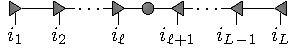
\includegraphics[valign=c]{figures/arbitrary_wavefunction_decomposed_decolorized.pdf}\ket{i_1,i_2,\dots,i_L}.
\end{align}
Please note that I use the sum convention in the above.
To cast \cref{eq:lagrangian_multiplier} into a variational problem for the tensors at position $\ell$ and $\ell+1$, it is convenient to use the graphical notation
\begin{align}
    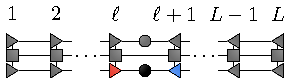
\includegraphics[valign=c]{figures/lagrangian_multiplier_equation_1.pdf}
    -
    \lambda_\psi
    \brlr{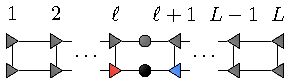
\includegraphics[valign=c]{figures/lagrangian_multiplier_equation_2.pdf}-1}
    =
    0.
    \label{eq:lagrangian_multiplier_graphical}
\end{align}
I now proceed by the application of a gradient on both sides of \cref{eq:lagrangian_multiplier}, in which case the elements correspond to the entries of the contraction of the red, black and blue tensor, i.e.
\begin{align}
    \nabla(\ell,\ell+1)_{kn}\equiv\frac\partial{\partial\brlr{U^{i_\ell}_{k,l}S_l V^{\dag i_{\ell+1}}_{l,n}}^*}.
\end{align}
Since the tensors enter in the equation in a linear fashion, the application of the gradient corresponds to removing the three tensors from the conjugate contraction (and of course the scalar $1$) in \cref{eq:lagrangian_multiplier_graphical}.
One finally arrives at
\begin{align}
    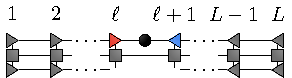
\includegraphics[valign=c]{figures/lagrangian_multiplier_equation_3.pdf}
    =
    \lambda_\psi
    
\includegraphics[valign=c]{figures/lagrangian_multiplier_equation_4.pdf}
    .
    \label{eq:lagrangian_multiplier_graphical_2}
\end{align}
This can be better understood after reshaping $U^{[\ell]}\Lambda V^{\dag[\ell+1]}$ (the red, black and blue tensors in \cref{eq:lagrangian_multiplier_graphical_2}) to a vector $v(\ell,\ell+1)=f\circ U^{[\ell]}\Lambda V^{\dag[\ell+1]}$ of dimension $m^2D^2$, in which $f$ denotes the reshaping.
The contracted network should then be reshaped to a matrix $h_{\rm eff.}(\ell,\ell+1)$ of dimension $m^2D^2\times m^2D^2$, such that
\begin{align}
    h_{\rm eff.}(\ell,\ell+1)v({\ell,\ell+1}) = \lambda_\psi v({\ell,\ell+1}).
    \label{eq:MPS_optimization}
\end{align}
The Lagrange multiplier $\lambda_\psi = v^\dag h_{\rm eff.} v / \sqrt{|v|^2}$ corresponds to the global energy of the MPS and the equations span a standard eigenvalue problem for the vector $v$ which can be solved efficiently for the end of the spectrum with libraries like ARPACK~\cite{Lehoucq1998}.
After the optimal low-energy vector $v$ is computed, it must be reshaped back to a tensor, and then decomposed through the generalized SVD to obtain the original canonical form of the MPS.
In particular, one performs the sequence
\begin{align}
    f^{-1}\circ v(\ell, \ell+1)
    \equiv
    
\includegraphics[valign=c]{figures/growing_4_4.pdf}
    =
    
\includegraphics[valign=c]{figures/growing_5.pdf}.
\end{align}
Note that the standard eigenvalue problem in \cref{eq:MPS_optimization} is promoted to a generalized eigenvalue problem if we would not rely on the normalized and canonical form of the MPS~\cite{Silvi2019}.
The aim now is to find the optimal vectors $v({\ell,\ell+1})$ for each site, which can be achieved in an iterative manner by the growing and finite MPS algorithm.
\\

A minimal example of the growing MPS algorithm is formalized as follows:
\begin{enumerate}
    \item Choose an even number $L$ corresponding to the final number of quantum numbers in the resulting quantum state.
    It is equal to twice the number of iterations.
    \item Set $n=1$. Compute the lowest energy vector $v(1,2)$ for a system of two sites only.
    The eigenvalue equation and graphical representation reads
    \begin{align}
        h_{\rm eff.} v(1,2) &= \lambda_\psi v(1,2)\\
        
\includegraphics[valign=c]{figures/two_site_problem_1.pdf},
        &=
        \lambda_\psi
        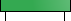
\includegraphics[valign=c]{figures/two_site_problem_2.pdf},
        \label{eq:two_site_problem}
    \end{align}
    in which the green tensor represents $v(1,2)$ and the two gray tensors correspond to the boundary tensors $W^{[1]}$ and $W^{[L]}$ representing the two-site Hamiltonian.
    % Note that the two green tensors can also be understood as rank-$3$ tensors in which the additional horizontal link has dimension $1$.
    \item Use the generalized singular value decomposition depicted in \cref{eq:SVD_generalized} to decouple the two quantum numbers into a product of two isometries and a matrix $\Lambda$ containing the spectral values
    \begin{align}
        v(1,2) &= U^{[i_1]}\Lambda V^{\dag[i_{L}]},
        \\
        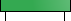
\includegraphics[valign=c]{figures/two_site_problem_2.pdf}
        &=
        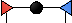
\includegraphics[valign=c]{figures/two_site_problem_2_decomp.pdf}.
    \end{align}
    Apply the compression of the tensor by keeping only the $m$ largest singular values, corresponding to the bond dimension.
    Renormalize the truncated matrix $\Lambda$ such that $\tr(\Lambda^2)=1$.
    \item Grow the size of the MPS from $2n$ to $2n+2$ sites by replacing the central matrix $\Lambda$ with a rank-$4$ tensor of fitting dimensions
    \begin{align}
        \brlr{\prod_{k=1}^nU^{[i_k]}}\Lambda \brlr{\prod_{k=1}^{n}V^{\dag[i_{L+1-n}]}}
        &\longrightarrow
        \brlr{\prod_{k=1}^nU^{[i_k]}} T^{[i_{n+1},i_{L-n}]}\brlr{\prod_{k=1}^{n}V^{\dag[i_{L+1-n}]}},
        \\
        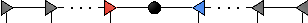
\includegraphics[valign=c]{figures/growing_4_1.pdf}
        &\longrightarrow
        
\includegraphics[valign=c]{figures/growing_4_2.pdf}
    \end{align}
    Then use \cref{eq:MPS_optimization} to variationally solve for the lowest energy vector $v(n+1,n+2)$ corresponding to the inserted tensor.
    \begin{align}
        h_{\rm eff.} v(n+1,2n+2) &= \lambda_\psi v(n+1,n+2)\\
        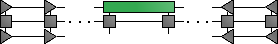
\includegraphics[valign=c]{figures/growing_4_3.pdf}
        &=
        \lambda_\psi
        
\includegraphics[valign=c]{figures/growing_4_4.pdf}.
        \label{eq:two_site_problem}
    \end{align}
    \item Use the generalized singular value decomposition to decouple the two quantum numbers into a product of two isometries and a matrix $\Lambda$ containing the spectral values
    \begin{align}
        v(n+1,n+2) &= U^{[i_{n+1}]}\Lambda V^{\dag[i_{L-n}]},
        \\
        
\includegraphics[valign=c]{figures/growing_4_4.pdf}
        &=
        
\includegraphics[valign=c]{figures/growing_5.pdf}.
    \end{align}
    Increase $n\rightarrow n+1$. Stop if $n=L/2$, else go back to step 4.
\end{enumerate}
The common application of the growing algorithm is two-fold.
It can be used naively to approximate the central tensors of a fully translationally invariant chain by sending $L\gg2$ to very large values.
The convergence is reached when the overlap between the optimal vectors $v(n,n+1)$ and $v(n-1,n)$ of the previous iteration step approaches a user-specified threshold.
This approach however requires the state to be fully translationally invariant over a single site.
A workaround of this issue is to relax the insertion of two sites in the center of the MPS to arbitrary many.
However, the convergence to the best thermodynamic MPS state is never achieved.
This is due to the intrinsically finite structure of the MPS in the growing algorithm which breaks translational symmetry at every step, and another Ansatz is required.
\\

One viable option is to approximate the (infinite) environments to the left and right of the central tensors with the dominant eigenstates of the transfer matrices.
The corresponding algorithm is then called infinite boundary conditioned MPS~\cite{phien2012} or variational uniform MPS (VUMPS)~\cite{zaunerstauber2018}.
In our works, we were mostly interested in the simulation of finite systems and I omit the description of such an implementation.
\\

The second application concerns the MPS obtained after $L/2$ steps -- it can serve as a trial state for a finite system of length $L$, which is then refined by the second algorithm, finite MPS:
\begin{enumerate}
    \item Set $n=1$. Start with a trial MPS in the canonical form (e.g. acquired by the growing algorithm) and transform the MPS such that the $\Lambda$ matrix is between sites $1$ and $2$, i.e.
    \begin{align}
        C^{i_1,i_2,i_3,\dots,i_{L-1},i_L} \equiv 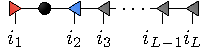
\includegraphics[valign=c]{figures/fMPS_1.pdf}.
    \end{align}
    \item Compute the lowest energy vector $v(n,n+1)$ according to \cref{eq:MPS_optimization} and decompose it to two isometries and a matrix $\Lambda$ containing the singular values
    \begin{align}
        v(n,n+1) \equiv U^{[i_n]}\Lambda(n) V^{\dag[i_{n+1}]}
        .
    \end{align}
    Proceed then with step $3$ (sweeping to the right) or $4$ (sweeping to the left).
    \item If $n=L-1$ continue with 4. Shift the matrix $\Lambda(n)$ to the next site by decomposing it to
    \begin{align}
        \Lambda(n) V^{\dag[i_{n+1}]} V^{\dag[i_{n+2}]} \rightarrow U^{[i_{n+1}]}\Lambda(n+1)\tilde V^{\dag[i_{n+2}]}
        .
    \end{align}
    Increase $n\rightarrow n+1$ and go back to step 2.
    This is called sweeping from left to right.
    \item If $n=1$ continue with 3. Shift the matrix $\Lambda(n)$ to the previous site by decomposing it to
    \begin{align}
        U^{[i_{n-1}]}U^{[i_n]}\Lambda(n) \rightarrow \tilde U^{[i_{n-1}]}\Lambda(n-1) V^{\dag[i_n]}
        .
    \end{align}
    Decrease $n\rightarrow n-1$ and go back to step 2.
    This is called sweeping from right to the left.
\end{enumerate}
The finite MPS optimization is usually performed in so-called ``sweeps'', i.e. a full sweeping cycle from left to right is done for each site $n=1,2,\dots,L-1$, after which a full sweeping cycle from right to left $n=L-1,L-2,\dots,1$ is applied.
Iteratively optimizing the local tensors leads to a variational trajectory in the manifold of MPS with bond dimension $m$.
\\

As usual, the precise representatives of global extrema in optimization schemes remain unknown and its always possible to be trapped inside of local minima.
In such cases, viable estimates of the error are needed.
The error to an exact eigenstate of the Hamiltonian can be estimated in a straightforward manner by computing the variance of the approximation.
For cases in which the MPS is equivalent to an eigenstate of the full Hamiltonian, the variance will reduce to $0$. In general, however, the approximation is not a true eigenstate of the Hamiltonian and as such we arrive at
\begin{align}
    \varepsilon(m) = \sqrt{\braket{\psi(m)|\hat H^2|\psi(m)} - \braket{\psi(m)|\hat H|\psi(m)}^2}\geq 0.
\end{align}
The indication of $m$ is reminiscent of the fact that in general, $\varepsilon$ depends on the bond dimension of the MPS.
It can then be checked that the variance converges to $0$ by performing a so-called bond dimension scaling analysis.
%
%
%%%%%%%%%%%%%%%%%%%%%%%%%%
\section{Time evolution}
\label{sec:time_evolution}
%%%%%%%%%%%%%%%%%%%%%%%%%%
%
%
%
%
%%%%%%%%%%%%%%%%%%%%%%%%%%%%%%%%%%%%%%%%%%%
\section{Entanglement and the area law}
\label{sec:entanglement_and_the_area_law}
%%%%%%%%%%%%%%%%%%%%%%%%%%%%%%%%%%%%%%%%%%%
All of the discussion so far would not be very exciting for a wholehearted physicist, were it not for its close relation to quantum entanglement.
The phenomenon was firstly noted in $1935$ by Albert Einstein, Boris Podolsky, and Nathan Rosen~\cite{EPR1935}, also Erwin Schrödinger~\cite{Schrdinger1935,Schrdinger1936}, describing what is famously known as the EPR paradox~\cite{Reid2009}.
At its heart, it describes a group of particles interacting such that the quantum state of each individual particle cannot be described independently of the state of the others in the group.
The paradox part in the aforementioned works is described by quantum measurements performed on individual particles, which leads to irreversible collapses of the wave function and an alteration of the original quantum state of the other particles in the group.
Surprisingly, the phenomenon is independent of the distance between the particles and forms thus a unique form of correlations exclusively present in quantum systems.
\\

To make an example, consider the two-particle pure state $\ket{\psi}=\frac1{\sqrt2}\brlr{\ket{\uparrow\downarrow}+\ket{\downarrow\uparrow}}$ and the two particles being localized at two distant spacial positions.
In case we prepare a projective measurement of the first particle being in the $\uparrow$-state, the probability of the outcome is obviously $1/2$ and we end up with a collapsed post-measurement state of the form $\ket{\tilde\psi} = \ket{\uparrow\downarrow}$.
At the time of the measurement, the second particle collapses to the perfectly correlated alignment, and it does so immediately, independent on the spacial distance between the two parties.
A subsequent measurement of the second particle will thus yield $\downarrow$ with probability $1$.
Note that this instantaneous action does not violate causality since the outcome of the first measurement is random and as such cannot be used to transmit information.
With this example in mind, let us now encapsulate the definition of $N$-partite separable and entangled for states with $N$ individual particles.
\\

A state $\ket{\psi}$ is called $N$-partite separable iff. it can be written as a product of $N$ subsystems~\cite{Horodecki2009}
\begin{align}
    \ket{\psi} = \ket{\psi_1}\otimes\ket{\psi_2}\otimes\dots\otimes\ket{\psi_N}.
    \label{eq:separable_states}
\end{align}
Note that this expression is fundamentally different from the coherent superposition of exponentially many state vectors encountered in generic states (compare to ~\cref{eq:generic_state}).
As such, we call a state entangled, if it cannot be decomposed according to~\cref{eq:separable_states}.
The earlier example of a bipartite system is an element of the Bell basis, which are sometimes called ERP states
\begin{align}
    \ket{\psi^\pm}=\frac 1{\sqrt2}\brlr{\ket{\uparrow\downarrow}\pm\ket{\downarrow\uparrow}}
    \quad
    \ket{\phi^\pm}=\frac 1{\sqrt2}\brlr{\ket{\uparrow\uparrow}\pm\ket{\downarrow\downarrow}}
\end{align}
and they all have remarkable properties, first recognized by Schrödinger -- if one measures only one of the states, one finds it with equal probability in either $\ket{0}$ or $\ket{1}$.
As such, they give no information about the subsystems, whereas they are still pure and thus reveal full information about the global system.
The Bell states are special cases of bipartite maximally entangled states~\cite{Horodecki2009} and as such great examples to explore the entropic manifestation of entanglement.
In particular, it has been shown that the von Neumann entropy of a subsystem can be greater than the entropy of the global system iff. the state is entangled~\cite{Horodecki1994}.
The inequality for separable states can thus be expressed as $S(B|A)=S(\hat\rho)-S(\hat\rho_{A/B})\geq0$ with $\hat\rho$ the density matrix and $\hat\rho_{A/B}$ the reduced density matrix of bipartition $A/B$.
As such, the von Neumann entropy serves as a scalar separability criteria, in analogy to the Bell inequalities.
The discussions of entangled states breaking the positivity of $S(A|B)$ reach far beyond the present aim of this introduction \cite{Horodecki2006}, and I simply conclude here that the von Neumann entropy is a useful scalar measure of bipartite entanglement.
\\

Coming back to the connection to MPS with finite bond dimension, we now know that the upper bound restriction of the entropy limits the available entanglement of the approximation.
This, in turn, does not provide an explanation why such an approximation should not ``go wrong quickly'' in a sense that the important properties of the approximated state are lost, even if the bond dimension is large.
Incidentally, at the time DMRG was introduced by Steven White~\cite{White1992}, the success of the renormalization scheme remained a mystery.
Some insights were concluded by the derivation of universal scaling laws of the entropy provided e.g. by Calabrese and Cardy in 2004~\cite{Calabrese2004} in proximity of a quantum critical point.
In 2007, Hastings published his famous proof of the area law for one-dimensional quantum systems~\cite{Hastings2007}.
In its essence, it provides an upper bound to the von Neumann entropy for gapped and local (i.e. no long-ranged interactions) Hamiltonians scaling as the area ($\equiv$ a constant) of one-dimensional systems.
Essentially, the works can be summarized by the following two statements~\cite{Eisert2010}:
Consider a block of $1,2,\dots,\ell$ particles with internal dimension $D$, the entanglement entropy scales as
\begin{align}
    S_1(\ell) &= \frac c{3b}\log[d(\ell)],\text{ if the system is critical}\\
    S_1(\ell) &= c_0\xi\log\brlr{6\xi}\log D2^{6\xi\log D},\text{ if the system is local and gapped $\Delta E>0$}
\end{align}
in which $c_0$ is a constant of order one, $\xi=\max(2v/\Delta E,\xi_C)$ is the correlation length, $v$ the velocity of sound, $\xi_C$ of order one and $d(\ell)$ encodes the size of the block.
For periodic ($b=1$) and open ($b=2$) boundary conditions, $d(\ell)$ is the chord distance encoding the length of a semi-circle
\begin{align}
    d(\ell) = \left|\frac L\pi\sin(\pi/L\ell)\right|.
\end{align}

% It has been until 1995 that the von Neumann entropy has been understood as the scalar value counting the number of quantum bits needed to transmit quantum states emitted by a statistical source~\cite{Schumacher1995}.

% The multiplication of the two coefficient functions is nothing but a tensor contraction of the legs $\bm q_B$.
% In particular, we may write
% \begin{align}
%     \sum_{\bm q_B}C(\bm i_A,\bm q_B)C^*(\bm j_A,\bm q_B)
%     \equiv
%     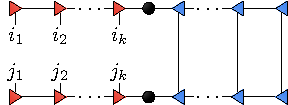
\includegraphics[valign=c]{figures/arbitrary_reduced_density_matrix_decomposed.pdf}.
% \end{align}
% Note that in the above, I conveniently used the canonical form of the MPS.
% As such, one may explore the isometry condition in \cref{eq:isometries}, resulting in the particularly appealing result
% \begin{align}
%     \sum_{\bm q_B}C(\bm i_A,\bm q_B)C^*(\bm j_A,\bm q_B)
%     \equiv
%     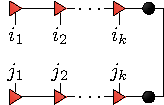
\includegraphics[valign=c]{figures/arbitrary_reduced_density_matrix_decomposed_simplified.pdf}.
% \end{align}
% Note that the isometrized canonical form allows to simplify the number of required contractions significantly, and
% \begin{align}
%     \sum_{\bm i_A, \bm j_A}\sum_{\bm q_B}C(\bm i_A,\bm q_B)C^*(\bm j_A,\bm q_B)\ket{\bm i_A}\bra{\bm j_A} = \sum_{\bm i'_A, \bm j'_A} S_k \ket{\bm i'_A}\bra{\bm j'_A}
% \end{align}
